\documentclass[conference]{IEEEtran}

\usepackage{graphicx}
\usepackage[]{hyperref}
\hypersetup{
    letterpaper,
    colorlinks,
    urlcolor=blue,
    linkcolor=blue,
    citecolor=blue,
}

\usepackage{url}
\usepackage{cite}

\bibliographystyle{IEEEtran}


% figure reference formatting
\newcommand{\figref}[1]{Fig.~\ref{#1}}


% TODO: check margins


\author{
    \IEEEauthorblockN{Daniel J. White\IEEEauthorrefmark{1},
        SatNOGS Developers\IEEEauthorrefmark{2}}
    \IEEEauthorblockA{\IEEEauthorrefmark{1}Valparaiso University, \href{mailto:dan.white@valpo.edu}{dan.white@valpo.edu}}
    \IEEEauthorblockA{\IEEEauthorrefmark{2}Libre Space Foundation,
    \href{mailto:info@satnogs.org}{info@satnogs.org}}
    
}

\title{SatNOGS: Satellite~Networked~Open~Ground~Station}

%TODO: add other authors



\begin{document}
\maketitle

\begin{abstract}
    TODO
\end{abstract}



\section{Introduction}
\IEEEPARstart{T}{he} SatNOGS\cite{SatNOGS} project seeks to build a full stack of open technologies for satellite ground stations.

Figure \figref{f:launches} shows that the number of CubeSat-class satellite launches has increased nearly exponentially since the first in 2000.
Previously the domain of University projects, the last 3 years have seen a huge increase in non-government or university launches.
These civilian satellites include commercial, like Planet Labs' Flock-1 satellites \cite{PlanetLabs}, non-profit, like The Planetary Society's recent LightSail \cite{PlanetarySociety}, and amateur, like AMSAT-NA's upcoming Fox-1 series \cite{AMSAT-NA}. 

Each satellite owner typically operates their own ground station for command and control.
The low-earth orbits (LEO) of these spacecraft result in short time windows when the spacecraft is above the local horizon for communication.
As a result, owners seek to enlist the help of other suitably equipped stations for collection of data.
The FUNcube project is a prime example of a well-organized effort to receive data from a satellite \cite{FUNcube}.

Recent advances in low-cost, software-defined radio (SDR) technology and 3D printing have put the construction within the reach of individuals.
Largely composed of Amateur Radio operators, these people receive telemetry and data from many satellites and provide the information to the owners and the general public.

What is missing is a way to connect these many owners and ground station operators in a way that is flexible and open.
The ESA's Global Educational Network for Satellite Operations \cite{GENSO}




\begin{figure}[htbp]
\centering
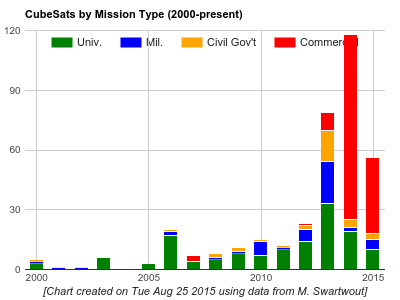
\includegraphics[width=\columnwidth]{fig/cubesat-launches}
\caption{CubeSat launches per year through 2015-07-17, from \cite{SwartwoutDatabase}.  The ``Commercial'' category includes non-profit and amateur satellites.}
\label{f:launches}
\end{figure}


\section{Network}

\section{Database}

\section{Client}

\section{Ground Station}

\section{Conclusion}

\bibliography{references}

\end{document}
% vim: spell wrap linebreak textwidth=0
